\documentclass[11pt, a4paper]{article}
\usepackage{graphicx, fullpage, hyperref, listings}
\usepackage{appendix, pdfpages, color}
\usepackage{indentfirst} %段首空两格 棒
\usepackage{chngpage} 
\usepackage{tocloft}            % This squashes the Table of Contents a bit
\usepackage{pdfpages}
\usepackage{multirow}
\usepackage{amsmath}
\usepackage{amssymb}
\usepackage{framed}
%\usepackage{math}
%% Used on windows
%\usepackage[UTF8]{ctex}
%\usepackage{array}%需要该宏包

%% Used On Ubuntu
\usepackage{CJKutf8}


\setlength\cftbeforesecskip{3pt}
\renewcommand{\contentsname}{\centerline{\textbf{Content}}}
\graphicspath{{images/}}

\usepackage{multicol}

\usepackage{graphicx}
\usepackage{epstopdf}
\hypersetup{CJKbookmarks,%
	bookmarksnumbered,%
	colorlinks,%
	linkcolor=black,%
	citecolor=black,%
	plainpages=false,%
	pdfstartview=FitH}

%%%%%%%代码语法高亮设置

\usepackage{color}

\definecolor{pblue}{rgb}{0.13,0.13,1}
\definecolor{pgreen}{rgb}{0,0.5,0}
\definecolor{pred}{rgb}{0.9,0,0}
\definecolor{pgrey}{rgb}{0.46,0.45,0.48}

\usepackage{listings}
\lstset{
	language=Java,
	showspaces=false,
	showtabs=false,
	%%%%%
	frame = single,
	stepnumber = 2,  
	numbersep = 4pt, 
	 numbers=left,
	%breakatwhitespace=false, 
	tabsize=2,  
	%%%%%
	breaklines=true,
	showstringspaces=false,
    breakatwhitespace=false, 
	commentstyle=\color{pgreen},
	keywordstyle=\color{pblue},
	stringstyle=\color{pred},
	basicstyle=\ttfamily,
	%moredelim=[il][\textcolor{pgrey}]{$$},
	%moredelim=[is][\textcolor{pgrey}]{\%\%}{\%\%},
}


%%%%%%%%代码语法高亮设置

\definecolor{MyLightYellow}{cmyk}{0,0.,0.2,0} 

\setlength{\parskip}{4pt}        % sets spacing between paragraphs
\interfootnotelinepenalty=500    % this prevents footnotes breaking across pages


\title{
\includegraphics[width=0.45\textwidth]{dg}
        \\Facial Expression Summary   }          % <<<<<<<<< change the title as appropriate
\author{Jiaming Nie}                    % <<<<<<<<< module code

\begin{document}
\begin{titlepage}
	
%\date{\today}
\maketitle
\addtocontents{toc}{\protect\thispagestyle{empty}}
% because we don't want a page number on the title page
% Thanks to Huang Shanyue for suggesting this 

%\date{\today}
\thispagestyle{empty}  %去除首页页码
%\tableofcontents

\end{titlepage}

%\tableofcontents
%\listoffigures

%\newpage


\begin{CJK}{UTF8}{gbsn}

\section{根据AffectNet Paper中对Train和Vali的划分}

AffectNet给出了一个测试集和验证集的划分,其中验证集中不同表情样本的数量是基本一致的。去除非表情的样本后,用GoogleNet得出的结果如下:

\subsection{Accuracy和Loss曲线}

Accuracy和Loss曲线可见于图\ref{fig:accuLoss}.

\begin{figure}[htbp]
	\centering %使插入的图片居中显示
	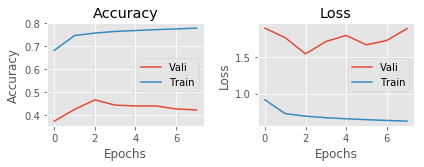
\includegraphics[width=10cm]{accuLoss}
	\caption{根据论文划分的Train和Vali 准确率和损失曲线}
	\label{fig:accuLoss}
	%插入图片的标题,一般放在图片的下方,放在表格的上方
\end{figure}

\subsection{相关结果}

在验证集上的结果如下:

\begin{table}[htbp] 
	\begin{center}
		\caption{ResNet18 在测试集的表现}
		\begin{tabular}{l | l}  \hline
			Accuracy  &  44.1265\%  \\ \hline
			Recall        &  0.441265 \\ \hline
			F1 Score    & 0.4011 \\ \hline
		\end{tabular}
		\label{tab:res18_test}
	\end{center}
\end{table}	

\subsection{Confusion Matrix}

在给定的Train Vali划分中,测试集中各个样板的比例较为均衡,具体的数如下:

\begin{table}[htbp] 
	\begin{center}
		\caption{给定划分数据集的Confusion Matrix}
		\begin{tabular}{ | l | l | l |  }  \hline
		Label & 数量 & 比例 \\ \hline
		Neutral  & 496   & 12.4\%    \\ \hline
		Happy  &  499 & 12.5\%  \\ \hline
		Sad   &  483  &  12.1\%  \\ \hline
		Surprise  & 497  & 12.5\%  \\ \hline
		Fear   &  498 &  12.5\% \\ \hline
		Disgust   &  501  &   12.6\%  \\ \hline
		Anger     &   497 & 12.5\%   \\ \hline
		Contempt   & 498   & 12.5\%   \\ \hline
		\end{tabular}
		\label{tab:occu}
	\end{center}
\end{table}	

Confusion matrix如下:
\begin{table}[htbp] 
	\begin{center}
		\caption{给定划分数据集的Confusion Matrix}
		\begin{tabular}{ | l | l | l | l | l |l | l |l | l | }  \hline
			实际/预测 &  Neutral  & Happy & Sad   &  Surprise   &  Fear  & Disgust  & Anger & Contempt  \\ \hline
			
			Neutral  & \textbf{0.829}  &  0.103  &  0.030  &  0.014  &  0.000  &  0.000  &  0.022  &  0.002 \\ \hline
			
			Happy   & 0.050  &  \textbf{0.944}  &  0.000  &  0.002  &  0.000  &  0.000  &  0.002  &  0.002 \\ \hline
			
			Sad    & 0.394  &  0.064  &  \textbf{0.482}  &  0.010  &  0.000  &  0.004  &  0.046  &  0.000  \\ \hline
			
			Surprise    &  0.404  &  0.187  &  0.030  &  \textbf{0.338}  &  0.018  &  0.002  &  0.020  &  0.000 \\ \hline
			
			Fear     &  0.279  &  0.070  &  0.104  &  0.245  &  \textbf{0.235}  &  0.006  &  0.060  &  0.000 \\ \hline
			
			Disgust      &   0.242  &  0.152  &  0.104  &  0.028  &  0.010  &  \textbf{0.178}  &  0.287  &  0.000 \\ \hline
			
			Anger       &  0.366  &  0.052  &  0.072  &  0.012  &  0.006  &  0.008  &  \textbf{0.479}  &  0.004 \\ \hline
			
			Contempt   & 0.351  &  0.544  &  0.010  &  0.006  &  0.000  &  0.002  &  0.038  &  \textbf{0.048} \\ \hline
		\end{tabular}
		\label{tab:res18_cm}
	\end{center}
\end{table}	

由Confusion Matrix看出,Neutral和Happy的预测准确率仍为最高,分别为82.9\%和94.4\%,此外Sad和Anger的准确率为48.2\%和47.9\%,接近50\%.

不同的表情被错误分类时,除contempt外,其他表情大多被错误预测为Neutral.

contempt标签54.4\%被预测为Happy,35.1\%被预测为Neutral.

\section{AlexNet验证的结果}

AffectNet Paper中给出的Baseline是使用了AlexNet并去除了contempt这个标签。

使用的模型参数和GoogleNet一致。Learning Rate 0.1, optimizer SGD, Epoch 8, Batch Size 16.

\subsection{Accuracy和Loss曲线}

Accuracy和Loss曲线可见于图\ref{fig:accuLoss}.

\begin{figure}[htbp]
	\centering %使插入的图片居中显示
	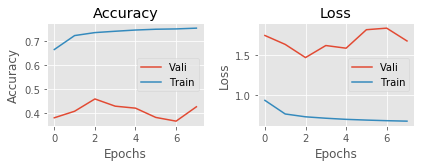
\includegraphics[width=10cm]{alexaccu}
	\caption{AlexNet的结果}
	\label{fig:alexaccu}
	%插入图片的标题,一般放在图片的下方,放在表格的上方
\end{figure}

\subsection{Confusion Matrix}

Confusion matrix如下:
\begin{table}[htbp] 
	\begin{center}
		\caption{AlexNet - Confusion Matrix}
		\begin{tabular}{ | l | l | l | l | l |l | l |l |  }  \hline
			实际/预测 &  Neutral  & Happy & Sad   &  Surprise   &  Fear  & Disgust  & Anger  \\ \hline
			
			Neutral  &  \textbf{0.761}  &  0.121  &  0.064  &  0.024  &  0.014  &  0.000  &  0.016 \\ \hline
			
			Happy   & 0.050  &  \textbf{0.926}  &  0.008  &  0.006  &  0.006  &  0.000  &  0.004  \\ \hline
			
			Sad    & 0.325  &  0.072  & \textbf{ 0.461}  &  0.016  &  0.064  &  0.000  &  0.062  \\ \hline
			
			Surprise  &  0.264  &  0.189  &  0.034  &  \textbf{0.404}  &  0.087  &  0.000  &  0.022  \\ \hline
			
			Fear     &  0.144  &  0.060  &  0.096  &  0.255  &  \textbf{0.391}  &  0.000  &  0.054 \\ \hline
			
			Disgust      &  0.260  &  0.162  &  0.136  &  0.036  &  0.054  &  0.064  &  0.288 \\ \hline
			
			Anger       &  0.349  &  0.050  &  0.068  &  0.024  &  0.040  &  0.004  &  \textbf{0.464} \\ \hline

		\end{tabular}
		\label{tab:alexnet_cm}
	\end{center}
\end{table}	

\section{AffectNet的其他结果}

在CVPR 2016上给出了AffectNet~\cite{ref:affcvpr}中7个基本标签的结果,比BaseLine整体提高了一些。Confusion Matrix可见与图~\ref{fig:affcm}.

\begin{figure}[htbp]
	\centering %使插入的图片居中显示
	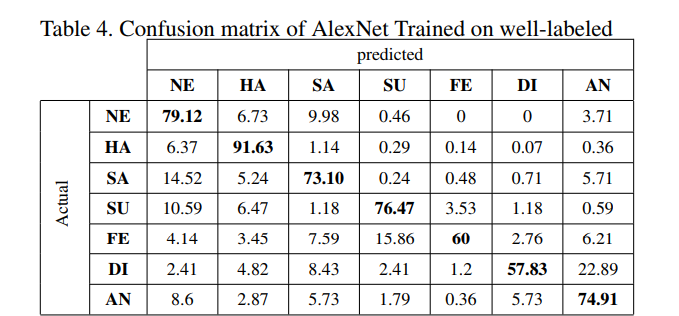
\includegraphics[width=15cm]{affcm}
	\caption{AffectNet 其他结果}
	\label{fig:affcm}
	%插入图片的标题,一般放在图片的下方,放在表格的上方
\end{figure}

\end{CJK}


%\tableofcontents

%\listoffigures
%\listoftables
%\lstlistoflistings        


%\newpage




\bibliographystyle{IEEEtran}  
\bibliography{MyRefs} 
\addcontentsline{toc}{section}{References}





%-------------------------------------------------------------------------------------------------------





\end{document}
